
% Default to the notebook output style

    


% Inherit from the specified cell style.




    
\documentclass[12pt]{extarticle}

    
    
%%%%%%%%%%%%%%%%%%%%%%%%%%%%%%%%%%%%%%%%%
% University Assignment Title Page LaTeX Template
% Version 1.0 (27/12/12)
%
% This template has been downloaded from:
% http://www.LaTeXTemplates.com
%
% Original author:
% WikiBooks (http://en.wikibooks.org/wiki/LaTeX/Title_Creation)
%
% License: CC BY-NC-SA 3.0 (http://creativecommons.org/licenses/by-nc-sa/3.0/)
% 
% Instructions for using this template:
% This title page is capable of being compiled as is. This is not useful for 
% including it in another document. To do this, you have two options: 
%
% 1) Copy/paste everything between \begin{document} and \end{document} 
% starting at \begin{titlepage} and paste this into another LaTeX file where you 
% want your title page.
% OR
% 2) Remove everything outside the \begin{titlepage} and \end{titlepage} and 
% move this file to the same directory as the LaTeX file you wish to add it to. 
% Then add \input{./title_page_1.tex} to your LaTeX file where you want your
% title page.
%
%%%%%%%%%%%%%%%%%%%%%%%%%%%%%%%%%%%%%%%%%
%\title{Title page with logo}
%----------------------------------------------------------------------------------------
%	PACKAGES AND OTHER DOCUMENT CONFIGURATIONS
%----------------------------------------------------------------------------------------

\usepackage[T1]{fontenc}
\usepackage{graphicx}
% We will generate all images so they have a width \maxwidth. This means
% that they will get their normal width if they fit onto the page, but
% are scaled down if they would overflow the margins.
\makeatletter
\def\maxwidth{\ifdim\Gin@nat@width>\linewidth\linewidth
\else\Gin@nat@width\fi}
\makeatother
\let\Oldincludegraphics\includegraphics
% Set max figure width to be 80% of text width, for now hardcoded.
\renewcommand{\includegraphics}[1]{\Oldincludegraphics[width=.8\maxwidth]{#1}}
% Ensure that by default, figures have no caption (until we provide a
% proper Figure object with a Caption API and a way to capture that
% in the conversion process - todo).
\usepackage{caption}
\DeclareCaptionLabelFormat{nolabel}{}
\captionsetup{labelformat=nolabel}

\usepackage{adjustbox} % Used to constrain images to a maximum size
\usepackage{xcolor} % Allow colors to be defined
\usepackage{enumerate} % Needed for markdown enumerations to work
\usepackage{geometry} % Used to adjust the document margins
\usepackage{amsmath} % Equations
\usepackage{amssymb} % Equations
\usepackage{textcomp} % defines textquotesingle
% Hack from http://tex.stackexchange.com/a/47451/13684:
\AtBeginDocument{%
    \def\PYZsq{\textquotesingle}% Upright quotes in Pygmentized code
}
\usepackage{upquote} % Upright quotes for verbatim code
\usepackage{eurosym} % defines \euro
\usepackage[mathletters]{ucs} % Extended unicode (utf-8) support
\usepackage[utf8x]{inputenc} % Allow utf-8 characters in the tex document
\usepackage{fancyvrb} % verbatim replacement that allows latex
\usepackage{grffile} % extends the file name processing of package graphics
                     % to support a larger range
% The hyperref package gives us a pdf with properly built
% internal navigation ('pdf bookmarks' for the table of contents,
% internal cross-reference links, web links for URLs, etc.)
\usepackage{hyperref}
\usepackage{booktabs}  % table support for pandoc > 1.12.2
\usepackage[inline]{enumitem} % IRkernel/repr support (it uses the enumerate* environment)
\usepackage[normalem]{ulem} % ulem is needed to support strikethroughs (\sout)
                            % normalem makes italics be italics, not underlines
\usepackage{braket}

%Cabeceras
\usepackage{fancyhdr}
\pagestyle{fancy}
\fancyhead[L]{MATERIA, AÑO}
\fancyhead[C]{}
\fancyhead[R]{UNPSJB}

\fancyfoot[R]{INTEGRANTES}
\fancyfoot[L]{TP}




    
    
    % Colors for the hyperref package
    \definecolor{urlcolor}{rgb}{0,.145,.698}
    \definecolor{linkcolor}{rgb}{.71,0.21,0.01}
    \definecolor{citecolor}{rgb}{.12,.54,.11}

    % ANSI colors
    \definecolor{ansi-black}{HTML}{3E424D}
    \definecolor{ansi-black-intense}{HTML}{282C36}
    \definecolor{ansi-red}{HTML}{E75C58}
    \definecolor{ansi-red-intense}{HTML}{B22B31}
    \definecolor{ansi-green}{HTML}{00A250}
    \definecolor{ansi-green-intense}{HTML}{007427}
    \definecolor{ansi-yellow}{HTML}{DDB62B}
    \definecolor{ansi-yellow-intense}{HTML}{B27D12}
    \definecolor{ansi-blue}{HTML}{208FFB}
    \definecolor{ansi-blue-intense}{HTML}{0065CA}
    \definecolor{ansi-magenta}{HTML}{D160C4}
    \definecolor{ansi-magenta-intense}{HTML}{A03196}
    \definecolor{ansi-cyan}{HTML}{60C6C8}
    \definecolor{ansi-cyan-intense}{HTML}{258F8F}
    \definecolor{ansi-white}{HTML}{C5C1B4}
    \definecolor{ansi-white-intense}{HTML}{A1A6B2}

    % commands and environments needed by pandoc snippets
    % extracted from the output of `pandoc -s`
    \providecommand{\tightlist}{%
      \setlength{\itemsep}{0pt}\setlength{\parskip}{0pt}}
    \DefineVerbatimEnvironment{Highlighting}{Verbatim}{commandchars=\\\{\}}
    % Add ',fontsize=\small' for more characters per line
    \newenvironment{Shaded}{}{}
    \newcommand{\KeywordTok}[1]{\textcolor[rgb]{0.00,0.44,0.13}{\textbf{{#1}}}}
    \newcommand{\DataTypeTok}[1]{\textcolor[rgb]{0.56,0.13,0.00}{{#1}}}
    \newcommand{\DecValTok}[1]{\textcolor[rgb]{0.25,0.63,0.44}{{#1}}}
    \newcommand{\BaseNTok}[1]{\textcolor[rgb]{0.25,0.63,0.44}{{#1}}}
    \newcommand{\FloatTok}[1]{\textcolor[rgb]{0.25,0.63,0.44}{{#1}}}
    \newcommand{\CharTok}[1]{\textcolor[rgb]{0.25,0.44,0.63}{{#1}}}
    \newcommand{\StringTok}[1]{\textcolor[rgb]{0.25,0.44,0.63}{{#1}}}
    \newcommand{\CommentTok}[1]{\textcolor[rgb]{0.38,0.63,0.69}{\textit{{#1}}}}
    \newcommand{\OtherTok}[1]{\textcolor[rgb]{0.00,0.44,0.13}{{#1}}}
    \newcommand{\AlertTok}[1]{\textcolor[rgb]{1.00,0.00,0.00}{\textbf{{#1}}}}
    \newcommand{\FunctionTok}[1]{\textcolor[rgb]{0.02,0.16,0.49}{{#1}}}
    \newcommand{\RegionMarkerTok}[1]{{#1}}
    \newcommand{\ErrorTok}[1]{\textcolor[rgb]{1.00,0.00,0.00}{\textbf{{#1}}}}
    \newcommand{\NormalTok}[1]{{#1}}
    
    % Additional commands for more recent versions of Pandoc
    \newcommand{\ConstantTok}[1]{\textcolor[rgb]{0.53,0.00,0.00}{{#1}}}
    \newcommand{\SpecialCharTok}[1]{\textcolor[rgb]{0.25,0.44,0.63}{{#1}}}
    \newcommand{\VerbatimStringTok}[1]{\textcolor[rgb]{0.25,0.44,0.63}{{#1}}}
    \newcommand{\SpecialStringTok}[1]{\textcolor[rgb]{0.73,0.40,0.53}{{#1}}}
    \newcommand{\ImportTok}[1]{{#1}}
    \newcommand{\DocumentationTok}[1]{\textcolor[rgb]{0.73,0.13,0.13}{\textit{{#1}}}}
    \newcommand{\AnnotationTok}[1]{\textcolor[rgb]{0.38,0.63,0.69}{\textbf{\textit{{#1}}}}}
    \newcommand{\CommentVarTok}[1]{\textcolor[rgb]{0.38,0.63,0.69}{\textbf{\textit{{#1}}}}}
    \newcommand{\VariableTok}[1]{\textcolor[rgb]{0.10,0.09,0.49}{{#1}}}
    \newcommand{\ControlFlowTok}[1]{\textcolor[rgb]{0.00,0.44,0.13}{\textbf{{#1}}}}
    \newcommand{\OperatorTok}[1]{\textcolor[rgb]{0.40,0.40,0.40}{{#1}}}
    \newcommand{\BuiltInTok}[1]{{#1}}
    \newcommand{\ExtensionTok}[1]{{#1}}
    \newcommand{\PreprocessorTok}[1]{\textcolor[rgb]{0.74,0.48,0.00}{{#1}}}
    \newcommand{\AttributeTok}[1]{\textcolor[rgb]{0.49,0.56,0.16}{{#1}}}
    \newcommand{\InformationTok}[1]{\textcolor[rgb]{0.38,0.63,0.69}{\textbf{\textit{{#1}}}}}
    \newcommand{\WarningTok}[1]{\textcolor[rgb]{0.38,0.63,0.69}{\textbf{\textit{{#1}}}}}
    
    
    % Define a nice break command that doesn't care if a line doesn't already
    % exist.
    \def\br{\hspace*{\fill} \\* }
    % Math Jax compatability definitions
    \def\gt{>}
    \def\lt{<}
    % Document parameters
    
    
    
    

    % Pygments definitions
    
\makeatletter
\def\PY@reset{\let\PY@it=\relax \let\PY@bf=\relax%
    \let\PY@ul=\relax \let\PY@tc=\relax%
    \let\PY@bc=\relax \let\PY@ff=\relax}
\def\PY@tok#1{\csname PY@tok@#1\endcsname}
\def\PY@toks#1+{\ifx\relax#1\empty\else%
    \PY@tok{#1}\expandafter\PY@toks\fi}
\def\PY@do#1{\PY@bc{\PY@tc{\PY@ul{%
    \PY@it{\PY@bf{\PY@ff{#1}}}}}}}
\def\PY#1#2{\PY@reset\PY@toks#1+\relax+\PY@do{#2}}

\expandafter\def\csname PY@tok@w\endcsname{\def\PY@tc##1{\textcolor[rgb]{0.73,0.73,0.73}{##1}}}
\expandafter\def\csname PY@tok@c\endcsname{\let\PY@it=\textit\def\PY@tc##1{\textcolor[rgb]{0.25,0.50,0.50}{##1}}}
\expandafter\def\csname PY@tok@cp\endcsname{\def\PY@tc##1{\textcolor[rgb]{0.74,0.48,0.00}{##1}}}
\expandafter\def\csname PY@tok@k\endcsname{\let\PY@bf=\textbf\def\PY@tc##1{\textcolor[rgb]{0.00,0.50,0.00}{##1}}}
\expandafter\def\csname PY@tok@kp\endcsname{\def\PY@tc##1{\textcolor[rgb]{0.00,0.50,0.00}{##1}}}
\expandafter\def\csname PY@tok@kt\endcsname{\def\PY@tc##1{\textcolor[rgb]{0.69,0.00,0.25}{##1}}}
\expandafter\def\csname PY@tok@o\endcsname{\def\PY@tc##1{\textcolor[rgb]{0.40,0.40,0.40}{##1}}}
\expandafter\def\csname PY@tok@ow\endcsname{\let\PY@bf=\textbf\def\PY@tc##1{\textcolor[rgb]{0.67,0.13,1.00}{##1}}}
\expandafter\def\csname PY@tok@nb\endcsname{\def\PY@tc##1{\textcolor[rgb]{0.00,0.50,0.00}{##1}}}
\expandafter\def\csname PY@tok@nf\endcsname{\def\PY@tc##1{\textcolor[rgb]{0.00,0.00,1.00}{##1}}}
\expandafter\def\csname PY@tok@nc\endcsname{\let\PY@bf=\textbf\def\PY@tc##1{\textcolor[rgb]{0.00,0.00,1.00}{##1}}}
\expandafter\def\csname PY@tok@nn\endcsname{\let\PY@bf=\textbf\def\PY@tc##1{\textcolor[rgb]{0.00,0.00,1.00}{##1}}}
\expandafter\def\csname PY@tok@ne\endcsname{\let\PY@bf=\textbf\def\PY@tc##1{\textcolor[rgb]{0.82,0.25,0.23}{##1}}}
\expandafter\def\csname PY@tok@nv\endcsname{\def\PY@tc##1{\textcolor[rgb]{0.10,0.09,0.49}{##1}}}
\expandafter\def\csname PY@tok@no\endcsname{\def\PY@tc##1{\textcolor[rgb]{0.53,0.00,0.00}{##1}}}
\expandafter\def\csname PY@tok@nl\endcsname{\def\PY@tc##1{\textcolor[rgb]{0.63,0.63,0.00}{##1}}}
\expandafter\def\csname PY@tok@ni\endcsname{\let\PY@bf=\textbf\def\PY@tc##1{\textcolor[rgb]{0.60,0.60,0.60}{##1}}}
\expandafter\def\csname PY@tok@na\endcsname{\def\PY@tc##1{\textcolor[rgb]{0.49,0.56,0.16}{##1}}}
\expandafter\def\csname PY@tok@nt\endcsname{\let\PY@bf=\textbf\def\PY@tc##1{\textcolor[rgb]{0.00,0.50,0.00}{##1}}}
\expandafter\def\csname PY@tok@nd\endcsname{\def\PY@tc##1{\textcolor[rgb]{0.67,0.13,1.00}{##1}}}
\expandafter\def\csname PY@tok@s\endcsname{\def\PY@tc##1{\textcolor[rgb]{0.73,0.13,0.13}{##1}}}
\expandafter\def\csname PY@tok@sd\endcsname{\let\PY@it=\textit\def\PY@tc##1{\textcolor[rgb]{0.73,0.13,0.13}{##1}}}
\expandafter\def\csname PY@tok@si\endcsname{\let\PY@bf=\textbf\def\PY@tc##1{\textcolor[rgb]{0.73,0.40,0.53}{##1}}}
\expandafter\def\csname PY@tok@se\endcsname{\let\PY@bf=\textbf\def\PY@tc##1{\textcolor[rgb]{0.73,0.40,0.13}{##1}}}
\expandafter\def\csname PY@tok@sr\endcsname{\def\PY@tc##1{\textcolor[rgb]{0.73,0.40,0.53}{##1}}}
\expandafter\def\csname PY@tok@ss\endcsname{\def\PY@tc##1{\textcolor[rgb]{0.10,0.09,0.49}{##1}}}
\expandafter\def\csname PY@tok@sx\endcsname{\def\PY@tc##1{\textcolor[rgb]{0.00,0.50,0.00}{##1}}}
\expandafter\def\csname PY@tok@m\endcsname{\def\PY@tc##1{\textcolor[rgb]{0.40,0.40,0.40}{##1}}}
\expandafter\def\csname PY@tok@gh\endcsname{\let\PY@bf=\textbf\def\PY@tc##1{\textcolor[rgb]{0.00,0.00,0.50}{##1}}}
\expandafter\def\csname PY@tok@gu\endcsname{\let\PY@bf=\textbf\def\PY@tc##1{\textcolor[rgb]{0.50,0.00,0.50}{##1}}}
\expandafter\def\csname PY@tok@gd\endcsname{\def\PY@tc##1{\textcolor[rgb]{0.63,0.00,0.00}{##1}}}
\expandafter\def\csname PY@tok@gi\endcsname{\def\PY@tc##1{\textcolor[rgb]{0.00,0.63,0.00}{##1}}}
\expandafter\def\csname PY@tok@gr\endcsname{\def\PY@tc##1{\textcolor[rgb]{1.00,0.00,0.00}{##1}}}
\expandafter\def\csname PY@tok@ge\endcsname{\let\PY@it=\textit}
\expandafter\def\csname PY@tok@gs\endcsname{\let\PY@bf=\textbf}
\expandafter\def\csname PY@tok@gp\endcsname{\let\PY@bf=\textbf\def\PY@tc##1{\textcolor[rgb]{0.00,0.00,0.50}{##1}}}
\expandafter\def\csname PY@tok@go\endcsname{\def\PY@tc##1{\textcolor[rgb]{0.53,0.53,0.53}{##1}}}
\expandafter\def\csname PY@tok@gt\endcsname{\def\PY@tc##1{\textcolor[rgb]{0.00,0.27,0.87}{##1}}}
\expandafter\def\csname PY@tok@err\endcsname{\def\PY@bc##1{\setlength{\fboxsep}{0pt}\fcolorbox[rgb]{1.00,0.00,0.00}{1,1,1}{\strut ##1}}}
\expandafter\def\csname PY@tok@kc\endcsname{\let\PY@bf=\textbf\def\PY@tc##1{\textcolor[rgb]{0.00,0.50,0.00}{##1}}}
\expandafter\def\csname PY@tok@kd\endcsname{\let\PY@bf=\textbf\def\PY@tc##1{\textcolor[rgb]{0.00,0.50,0.00}{##1}}}
\expandafter\def\csname PY@tok@kn\endcsname{\let\PY@bf=\textbf\def\PY@tc##1{\textcolor[rgb]{0.00,0.50,0.00}{##1}}}
\expandafter\def\csname PY@tok@kr\endcsname{\let\PY@bf=\textbf\def\PY@tc##1{\textcolor[rgb]{0.00,0.50,0.00}{##1}}}
\expandafter\def\csname PY@tok@bp\endcsname{\def\PY@tc##1{\textcolor[rgb]{0.00,0.50,0.00}{##1}}}
\expandafter\def\csname PY@tok@fm\endcsname{\def\PY@tc##1{\textcolor[rgb]{0.00,0.00,1.00}{##1}}}
\expandafter\def\csname PY@tok@vc\endcsname{\def\PY@tc##1{\textcolor[rgb]{0.10,0.09,0.49}{##1}}}
\expandafter\def\csname PY@tok@vg\endcsname{\def\PY@tc##1{\textcolor[rgb]{0.10,0.09,0.49}{##1}}}
\expandafter\def\csname PY@tok@vi\endcsname{\def\PY@tc##1{\textcolor[rgb]{0.10,0.09,0.49}{##1}}}
\expandafter\def\csname PY@tok@vm\endcsname{\def\PY@tc##1{\textcolor[rgb]{0.10,0.09,0.49}{##1}}}
\expandafter\def\csname PY@tok@sa\endcsname{\def\PY@tc##1{\textcolor[rgb]{0.73,0.13,0.13}{##1}}}
\expandafter\def\csname PY@tok@sb\endcsname{\def\PY@tc##1{\textcolor[rgb]{0.73,0.13,0.13}{##1}}}
\expandafter\def\csname PY@tok@sc\endcsname{\def\PY@tc##1{\textcolor[rgb]{0.73,0.13,0.13}{##1}}}
\expandafter\def\csname PY@tok@dl\endcsname{\def\PY@tc##1{\textcolor[rgb]{0.73,0.13,0.13}{##1}}}
\expandafter\def\csname PY@tok@s2\endcsname{\def\PY@tc##1{\textcolor[rgb]{0.73,0.13,0.13}{##1}}}
\expandafter\def\csname PY@tok@sh\endcsname{\def\PY@tc##1{\textcolor[rgb]{0.73,0.13,0.13}{##1}}}
\expandafter\def\csname PY@tok@s1\endcsname{\def\PY@tc##1{\textcolor[rgb]{0.73,0.13,0.13}{##1}}}
\expandafter\def\csname PY@tok@mb\endcsname{\def\PY@tc##1{\textcolor[rgb]{0.40,0.40,0.40}{##1}}}
\expandafter\def\csname PY@tok@mf\endcsname{\def\PY@tc##1{\textcolor[rgb]{0.40,0.40,0.40}{##1}}}
\expandafter\def\csname PY@tok@mh\endcsname{\def\PY@tc##1{\textcolor[rgb]{0.40,0.40,0.40}{##1}}}
\expandafter\def\csname PY@tok@mi\endcsname{\def\PY@tc##1{\textcolor[rgb]{0.40,0.40,0.40}{##1}}}
\expandafter\def\csname PY@tok@il\endcsname{\def\PY@tc##1{\textcolor[rgb]{0.40,0.40,0.40}{##1}}}
\expandafter\def\csname PY@tok@mo\endcsname{\def\PY@tc##1{\textcolor[rgb]{0.40,0.40,0.40}{##1}}}
\expandafter\def\csname PY@tok@ch\endcsname{\let\PY@it=\textit\def\PY@tc##1{\textcolor[rgb]{0.25,0.50,0.50}{##1}}}
\expandafter\def\csname PY@tok@cm\endcsname{\let\PY@it=\textit\def\PY@tc##1{\textcolor[rgb]{0.25,0.50,0.50}{##1}}}
\expandafter\def\csname PY@tok@cpf\endcsname{\let\PY@it=\textit\def\PY@tc##1{\textcolor[rgb]{0.25,0.50,0.50}{##1}}}
\expandafter\def\csname PY@tok@c1\endcsname{\let\PY@it=\textit\def\PY@tc##1{\textcolor[rgb]{0.25,0.50,0.50}{##1}}}
\expandafter\def\csname PY@tok@cs\endcsname{\let\PY@it=\textit\def\PY@tc##1{\textcolor[rgb]{0.25,0.50,0.50}{##1}}}

\def\PYZbs{\char`\\}
\def\PYZus{\char`\_}
\def\PYZob{\char`\{}
\def\PYZcb{\char`\}}
\def\PYZca{\char`\^}
\def\PYZam{\char`\&}
\def\PYZlt{\char`\<}
\def\PYZgt{\char`\>}
\def\PYZsh{\char`\#}
\def\PYZpc{\char`\%}
\def\PYZdl{\char`\$}
\def\PYZhy{\char`\-}
\def\PYZsq{\char`\'}
\def\PYZdq{\char`\"}
\def\PYZti{\char`\~}
% for compatibility with earlier versions
\def\PYZat{@}
\def\PYZlb{[}
\def\PYZrb{]}
\makeatother


    % Exact colors from NB
    \definecolor{incolor}{rgb}{0.0, 0.0, 0.5}
    \definecolor{outcolor}{rgb}{0.545, 0.0, 0.0}



    
    % Prevent overflowing lines due to hard-to-break entities
    \sloppy 
    % Setup hyperref package
    \hypersetup{
      breaklinks=true,  % so long urls are correctly broken across lines
      colorlinks=true,
      urlcolor=urlcolor,
      linkcolor=linkcolor,
      citecolor=citecolor,
      }
    % Slightly bigger margins than the latex defaults
    
    \geometry{verbose,tmargin=1in,bmargin=1in,lmargin=1in,rmargin=1in}
    
    

    \begin{document}
    
    
    
\begin{titlepage}

    \newcommand{\HRule}{\rule{\linewidth}{0.5mm}} % Defines a new command for the horizontal lines, change thickness here

    \center % Center everything on the page
     
    %----------------------------------------------------------------------------------------
    %	HEADING SECTIONS
    %----------------------------------------------------------------------------------------

    \textsc{\LARGE UNPSJB}\\[1cm] % Name of your university/college
    \textsc{\Large -Licenciatura en Sistemas OGCPI-}\\[0.5cm] % Major heading such as course name
    \textsc{\large -Sistemas Distribuidos-}\\[0.5cm] % Minor heading such as course title

    %----------------------------------------------------------------------------------------
    %	TITLE SECTION
    %----------------------------------------------------------------------------------------

    \HRule \\[0.4cm]
    {\huge \bfseries -Trabajo de Laboratorio 4-}\\[0.4cm] % Title of your document
    {\large \bfseries -Código Móvil. Comunicación Indirecta. MQTT. IoT-}\\[0.4cm] % Title of your document
    \HRule \\[1.5cm]
     
    %----------------------------------------------------------------------------------------
    %	AUTHOR SECTION
    %----------------------------------------------------------------------------------------


    \begin{minipage}[l]{0.5\textwidth}
        \begin{flushleft}
            \textbf{\textsf{Cátedra}}\\
            \large Mg. Ing Ricardo López\\ 
            \large Lic. Cristian Parise\\ 
            \linespread{4}
            \end{flushleft}
    \end{minipage}
    \begin{minipage}[l]{0.4\textwidth}
        \begin{flushright}
            \textbf{\textsf{Integrantes:}}\\
            \linespread{1}
            \large Lucas Krmpotic\\
            \large Maximiliano Águila\\
        \end{flushright}
    \end{minipage}\\[1.5cm]

    % If you don't want a supervisor, uncomment the two lines below and remove the section above
    %\Large \emph{Author:}\\
    %John \textsc{Smith}\\[3cm] % Your name

    %----------------------------------------------------------------------------------------
    %	DATE SECTION
    %----------------------------------------------------------------------------------------

    {\large \today}\\[1cm] % Date, change the \today to a set date if you want to be precise

    %----------------------------------------------------------------------------------------
    %	LOGO SECTION
    %----------------------------------------------------------------------------------------
    \begin{center}
    \adjustimage{max size={0.9\linewidth}{0.9\paperheight}}{images/logoUnpsjb.png}
    \end{center}
    { \hspace*{\fill} \\}
%    \includegraphics[scale=1]{./}\\[0.5cm] % Include a department/university logo - this will require the graphicx package
     
    %----------------------------------------------------------------------------------------

    % \vfill % Fill the rest of the page with whitespace

\end{titlepage}

\newpage
\tableofcontents
\newpage

    
    

    
    \section{Desarrolle un experimento (mediante Telnet o analizador de
paquetes) que muestre si el servidor de HTTP agrega o quita información
a la que genera un programa CGI. Nota: debería programar o utilizar un
programa CGI para conocer exactamente lo que genera y debería mostrar la
información que llega del lado del cliente, a nivel de HTTP o HTML
(preferentemente
HTTP).}\label{desarrolle-un-experimento-mediante-telnet-o-analizador-de-paquetes-que-muestre-si-el-servidor-de-http-agrega-o-quita-informaciuxf3n-a-la-que-genera-un-programa-cgi.-nota-deberuxeda-programar-o-utilizar-un-programa-cgi-para-conocer-exactamente-lo-que-genera-y-deberuxeda-mostrar-la-informaciuxf3n-que-llega-del-lado-del-cliente-a-nivel-de-http-o-html-preferentemente-http.}

    \subsection{Experimento con modulo "requests" de
python}\label{experimento-con-modulo-requests-de-python}

    La aplicación cgi para este ejercicio se encuentra en
\emph{"1/cgi-bin/hola.py"}

    CGI gestiona las cabeceras http que no definimos explícitamente y que
son necesarias para lograr una respuesta consistente, que sea aceptada
por el cliente.

En el siguiente ejemplo se muestran las cabeceras de la petición y de la
respuesta (de la cual solo se definió explícitamente el Content-type) y
el texto de la respuesta.

    \begin{Verbatim}[commandchars=\\\{\}]
{\color{incolor}In [{\color{incolor}7}]:} \PY{k+kn}{import} \PY{n+nn}{requests}
        \PY{k+kn}{import} \PY{n+nn}{json}
        \PY{n}{response} \PY{o}{=} \PY{n}{requests}\PY{o}{.}\PY{n}{post}\PY{p}{(}\PY{l+s+s2}{\PYZdq{}}\PY{l+s+s2}{http://localhost:8080/cgi\PYZhy{}bin/hola.py}\PY{l+s+s2}{\PYZdq{}}\PY{p}{)}
        \PY{n+nb}{print}\PY{p}{(}\PY{l+s+s2}{\PYZdq{}}\PY{l+s+s2}{\PYZhy{}\PYZhy{}\PYZhy{}\PYZhy{}\PYZhy{}\PYZhy{}\PYZhy{}\PYZhy{}\PYZhy{}\PYZhy{}\PYZhy{}\PYZhy{} cabeceras de la petición \PYZhy{}\PYZhy{}\PYZhy{}\PYZhy{}\PYZhy{}\PYZhy{}\PYZhy{}\PYZhy{}\PYZhy{}\PYZhy{}\PYZhy{}\PYZhy{}\PYZhy{}\PYZhy{}\PYZhy{}\PYZhy{}}\PY{l+s+s2}{\PYZdq{}}\PY{p}{)}
        \PY{n+nb}{print}\PY{p}{(}\PY{p}{)}
        \PY{n+nb}{print}\PY{p}{(}\PY{n}{json}\PY{o}{.}\PY{n}{dumps}\PY{p}{(}\PY{n+nb}{dict}\PY{p}{(}\PY{n}{response}\PY{o}{.}\PY{n}{request}\PY{o}{.}\PY{n}{headers}\PY{p}{)}\PY{p}{,} \PY{n}{indent}\PY{o}{=}\PY{l+m+mi}{2}\PY{p}{)}\PY{p}{)}
        
        \PY{n+nb}{print}\PY{p}{(}\PY{l+s+s2}{\PYZdq{}}\PY{l+s+s2}{\PYZhy{}\PYZhy{}\PYZhy{}\PYZhy{}\PYZhy{}\PYZhy{}\PYZhy{}\PYZhy{}\PYZhy{}\PYZhy{}\PYZhy{}\PYZhy{} cabeceras de la respuesta \PYZhy{}\PYZhy{}\PYZhy{}\PYZhy{}\PYZhy{}\PYZhy{}\PYZhy{}\PYZhy{}\PYZhy{}\PYZhy{}\PYZhy{}\PYZhy{}\PYZhy{}\PYZhy{}\PYZhy{}\PYZhy{}}\PY{l+s+s2}{\PYZdq{}}\PY{p}{)}
        \PY{n+nb}{print}\PY{p}{(}\PY{p}{)}
        \PY{n+nb}{print}\PY{p}{(}\PY{n}{json}\PY{o}{.}\PY{n}{dumps}\PY{p}{(}\PY{n+nb}{dict}\PY{p}{(}\PY{n}{response}\PY{o}{.}\PY{n}{headers}\PY{p}{)}\PY{p}{,} \PY{n}{indent}\PY{o}{=}\PY{l+m+mi}{2}\PY{p}{)}\PY{p}{)}
        
        \PY{n+nb}{print}\PY{p}{(}\PY{l+s+s2}{\PYZdq{}}\PY{l+s+s2}{\PYZhy{}\PYZhy{}\PYZhy{}\PYZhy{}\PYZhy{}\PYZhy{}\PYZhy{}\PYZhy{}\PYZhy{}\PYZhy{}\PYZhy{}\PYZhy{} texto de la respuesta \PYZhy{}\PYZhy{}\PYZhy{}\PYZhy{}\PYZhy{}\PYZhy{}\PYZhy{}\PYZhy{}\PYZhy{}\PYZhy{}\PYZhy{}\PYZhy{}\PYZhy{}\PYZhy{}\PYZhy{}\PYZhy{}}\PY{l+s+s2}{\PYZdq{}}\PY{p}{)}
        \PY{n+nb}{print}\PY{p}{(}\PY{p}{)}
        \PY{n+nb}{print}\PY{p}{(}\PY{n}{response}\PY{o}{.}\PY{n}{text}\PY{p}{)}
\end{Verbatim}


    \begin{Verbatim}[commandchars=\\\{\}]
------------ cabeceras de la petición ----------------

\{
  "User-Agent": "python-requests/2.20.1",
  "Accept-Encoding": "gzip, deflate",
  "Accept": "*/*",
  "Connection": "keep-alive",
  "Content-Length": "0"
\}
------------ cabeceras de la respuesta ----------------

\{
  "Date": "Sun, 11 Nov 2018 18:06:31 GMT",
  "Server": "Apache/2.4.35 (Unix)",
  "Keep-Alive": "timeout=5, max=100",
  "Connection": "Keep-Alive",
  "Transfer-Encoding": "chunked",
  "Content-Type": "text/html"
\}
------------ texto de la respuesta ----------------


<HTML><head><title>CGI</title></head><BODY>

<font color = blue>

<TITLE>CGI script output</TITLE>
<h1 style="TEXT-ALIGN: center">HOLA MUNDO</h1>

</font>

</HTML>


    \end{Verbatim}

    Por otro lado también un contenido html de las respuestas de error

    \begin{Verbatim}[commandchars=\\\{\}]
{\color{incolor}In [{\color{incolor}11}]:} \PY{n}{response} \PY{o}{=} \PY{n}{requests}\PY{o}{.}\PY{n}{post}\PY{p}{(}\PY{l+s+s2}{\PYZdq{}}\PY{l+s+s2}{http://localhost:8080/cgi\PYZhy{}bin/algoquenoexiste.py}\PY{l+s+s2}{\PYZdq{}}\PY{p}{)}
         \PY{n+nb}{print}\PY{p}{(}\PY{l+s+s2}{\PYZdq{}}\PY{l+s+s2}{\PYZhy{}\PYZhy{}\PYZhy{}\PYZhy{}\PYZhy{}\PYZhy{}\PYZhy{}\PYZhy{}\PYZhy{}\PYZhy{}\PYZhy{}\PYZhy{} cabeceras de la respuesta \PYZhy{}\PYZhy{}\PYZhy{}\PYZhy{}\PYZhy{}\PYZhy{}\PYZhy{}\PYZhy{}\PYZhy{}\PYZhy{}\PYZhy{}\PYZhy{}\PYZhy{}\PYZhy{}\PYZhy{}\PYZhy{}}\PY{l+s+s2}{\PYZdq{}}\PY{p}{)}
         \PY{n+nb}{print}\PY{p}{(}\PY{p}{)}
         \PY{n+nb}{print}\PY{p}{(}\PY{n}{json}\PY{o}{.}\PY{n}{dumps}\PY{p}{(}\PY{n+nb}{dict}\PY{p}{(}\PY{n}{response}\PY{o}{.}\PY{n}{headers}\PY{p}{)}\PY{p}{,} \PY{n}{indent}\PY{o}{=}\PY{l+m+mi}{2}\PY{p}{)}\PY{p}{)}
         
         \PY{n+nb}{print}\PY{p}{(}\PY{l+s+s2}{\PYZdq{}}\PY{l+s+s2}{\PYZhy{}\PYZhy{}\PYZhy{}\PYZhy{}\PYZhy{}\PYZhy{}\PYZhy{}\PYZhy{}\PYZhy{}\PYZhy{}\PYZhy{}\PYZhy{} texto de la respuesta \PYZhy{}\PYZhy{}\PYZhy{}\PYZhy{}\PYZhy{}\PYZhy{}\PYZhy{}\PYZhy{}\PYZhy{}\PYZhy{}\PYZhy{}\PYZhy{}\PYZhy{}\PYZhy{}\PYZhy{}\PYZhy{}}\PY{l+s+s2}{\PYZdq{}}\PY{p}{)}
         \PY{n+nb}{print}\PY{p}{(}\PY{p}{)}
         \PY{n+nb}{print}\PY{p}{(}\PY{n}{response}\PY{o}{.}\PY{n}{text}\PY{p}{)}
\end{Verbatim}


    \begin{Verbatim}[commandchars=\\\{\}]
------------ cabeceras de la respuesta ----------------

\{
  "Date": "Sun, 11 Nov 2018 18:10:15 GMT",
  "Server": "Apache/2.4.35 (Unix)",
  "Vary": "accept-language,accept-charset",
  "Accept-Ranges": "bytes",
  "Keep-Alive": "timeout=5, max=100",
  "Connection": "Keep-Alive",
  "Transfer-Encoding": "chunked",
  "Content-Type": "text/html; charset=utf-8",
  "Content-Language": "en"
\}
------------ texto de la respuesta ----------------

<?xml version="1.0" encoding="UTF-8"?>
<!DOCTYPE html PUBLIC "-//W3C//DTD XHTML 1.0 Strict//EN"
  "http://www.w3.org/TR/xhtml1/DTD/xhtml1-strict.dtd">
<html xmlns="http://www.w3.org/1999/xhtml" lang="en" xml:lang="en">
<head>
<title>Object not found!</title>
<link rev="made" href="mailto:you@example.com" />
<style type="text/css"><!--/*--><![CDATA[/*><!--*/ 
    body \{ color: \#000000; background-color: \#FFFFFF; \}
    a:link \{ color: \#0000CC; \}
    p, address \{margin-left: 3em;\}
    span \{font-size: smaller;\}
/*]]>*/--></style>
</head>

<body>
<h1>Object not found!</h1>
<p>


    The requested URL was not found on this server.

  

    If you entered the URL manually please check your
    spelling and try again.

  

</p>
<p>
If you think this is a server error, please contact
the <a href="mailto:you@example.com">webmaster</a>.

</p>

<h2>Error 404</h2>
<address>
  <a href="/">localhost</a><br />
  <span>Apache/2.4.35 (Unix)</span>
</address>
</body>
</html>



    \end{Verbatim}

    \subsection{Experimento desde
Wireshark}\label{experimento-desde-wireshark}

\begin{figure}[h]
\centering
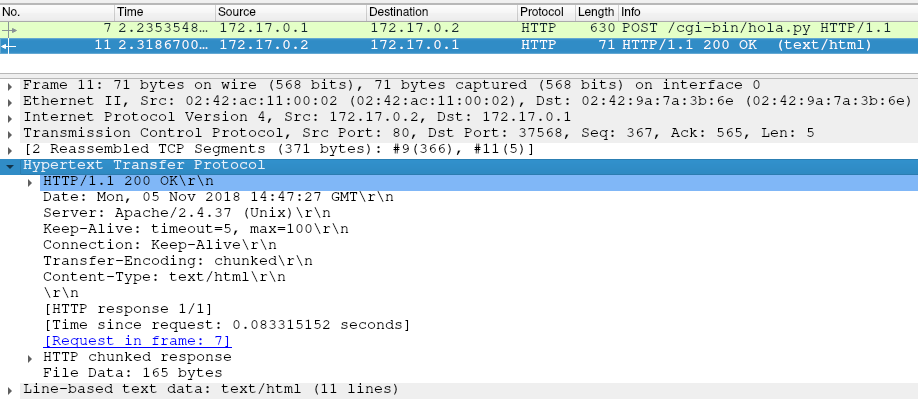
\includegraphics{images/pto1.png}
\caption{}
\end{figure}

    \subsection{Conclusion}\label{conclusion}

Analizando el header, podemos ver que a nivel HTTP se agregan los campos
de estado, fecha, servidor y última modificación.

    \section{Se debe desarrollar una aplicación que presente al usuario una
página web con una opción de carga de datos y una opción de modificación
de datos. La opción de carga consistirá en mostrar un formulario con un
conjunto de datos a completar y que luego almacene estos datos en un
archivo de texto plano. Los datos
son:}\label{se-debe-desarrollar-una-aplicaciuxf3n-que-presente-al-usuario-una-puxe1gina-web-con-una-opciuxf3n-de-carga-de-datos-y-una-opciuxf3n-de-modificaciuxf3n-de-datos.-la-opciuxf3n-de-carga-consistiruxe1-en-mostrar-un-formulario-con-un-conjunto-de-datos-a-completar-y-que-luego-almacene-estos-datos-en-un-archivo-de-texto-plano.-los-datos-son}

\begin{itemize}
\item
  Nombre y Apellido (hasta 70 caracteres)
\item
  Número de Alumno/Legajo (cantidad de dígitos limitada)
\item
  Sexo (lista desplegable para elegir entre Masculino o Femenino)
\item
  Edad (hasta dos dígitos)
\item
  Contraseña (que no se muestre en pantalla)
\end{itemize}

Para el caso de ``modificación'', se deberá requerir Numero de Alumno y
la Contraseña, si este par es encontrado en el archivo de texto plano,
se muestra lo que ya se tiene para ser modificado como si se estuvieran
cargando los datos, pero con los valores iniciales/default cargados del
archivo. Utilizar cookies para permitir sucesivas modificaciones sobre
los datos sin volver a pedir el legajo y palabra clave.

Se deben desarrollar las páginas estáticas HTML, el o los programas CGI
para procesar los datos y la distribución de estos componentes en el
sistema de archivos.

Justifique si este ejercicio puede ser considerado una aplicación web.

    \subsection{Implementacion}\label{implementacion}

Para la implementacion del \textbf{Servidor} utilizamos el modemo MVC
(Model, View, Controller) para un manejo claro de la funcionalidad.

\begin{figure}
\centering
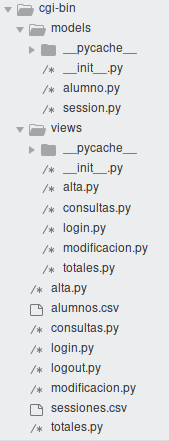
\includegraphics{images/Servidor_completo.png}
\caption{}
\end{figure}

Donde los archivos: + login.py + logout.py + alta.py + modificacion.py +
consultas.py + totales.py

Son los \textbf{Controladores} y los archivos dentro de la carpeta
\textbf{Models} son el \textbf{Modelo} y los archivos dentro de la
carpeta \textbf{Views} son nuestras \textbf{Vistas}.

Luego en la carpet \textbf{html} tenemos solamente una plantilla html,
\textbf{index.html}.

\begin{figure}[h]
\centering
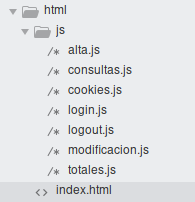
\includegraphics{images/html.png}
\caption{}
\end{figure}

Esto es asi y no tenemos las demas plantillas, porque utilizamos
\textbf{AJAX} para formar y armar el contenido de la pagina. Según la
peticion requerida, se va insertando en el container de la pagina los
distintos htmls.

Dentro del directorio \textbf{js} tenemos los archivos javascript con
las peticiones que realizara el navegador a nuestro servidor.

El controlador a esta accion, verifica si la peticion es un \textbf{GET}
o un \textbf{POST} y segun esto realiza una determinada funcion.

El \textbf{Controlador} verifica el \textbf{GET} o \textbf{POST} de la
siguiente manera:

\begin{Shaded}
\begin{Highlighting}[]
\ControlFlowTok{if}\NormalTok{ os.environ[}\StringTok{"REQUEST_METHOD"}\NormalTok{] }\OperatorTok{==} \StringTok{"POST"}\NormalTok{:}
    \CommentTok{# Accion al POST}

\ControlFlowTok{if}\NormalTok{ os.environ[}\StringTok{"REQUEST_METHOD"}\NormalTok{] }\OperatorTok{==} \StringTok{"GET"}\NormalTok{:}
    \CommentTok{# Accion al GET}
\end{Highlighting}
\end{Shaded}

Otra desicion que se tomo, fue la de utilizar archivos CSV para menejar
las sesiones y los alumnos dados de alta.

Para manejar este tipo de archivo utilizamos la libreria de python
\textbf{pandas} que nos brinda un manejo mas transparente y no tan
rudimentario de este tipo de archivos (csv).

Como ventaja de esta libreria, pudimos manipular mas facilmente los
archivos csv sin necesitar de bucles para las consultas. Un claro
ejemplo de utilizacion en nuestro proyecto es en la clase
\textbf{alumno.py} del \textbf{modelo} con su metodo
\textbf{get\_totales()}.

\begin{Shaded}
\begin{Highlighting}[]
\KeywordTok{def}\NormalTok{ get_totales(cls):}
\NormalTok{    alumnos }\OperatorTok{=}\NormalTok{ pd.read_csv(MODEL_FILE)}

\NormalTok{    result }\OperatorTok{=}\NormalTok{ \{}
        \StringTok{"mujeres1"}\NormalTok{:}\BuiltInTok{len}\NormalTok{(alumnos[(alumnos[}\StringTok{'sexo'}\NormalTok{] }\OperatorTok{==} \StringTok{"femenino"}\NormalTok{) }\OperatorTok{&} \OperatorTok{\textbackslash{}}
\NormalTok{                               (alumnos[}\StringTok{'edad'}\NormalTok{] }\OperatorTok{<} \DecValTok{21}\NormalTok{)]),}
        \StringTok{"mujeres2"}\NormalTok{:}\BuiltInTok{len}\NormalTok{(alumnos[(alumnos[}\StringTok{'sexo'}\NormalTok{] }\OperatorTok{==} \StringTok{"femenino"}\NormalTok{) }\OperatorTok{&} \OperatorTok{\textbackslash{}}
\NormalTok{                               ((alumnos[}\StringTok{'edad'}\NormalTok{] }\OperatorTok{>} \DecValTok{20}\NormalTok{) }\OperatorTok{&}\NormalTok{ (alumnos[}\StringTok{'edad'}\NormalTok{] }\OperatorTok{<} \DecValTok{41}\NormalTok{))]),}
        \StringTok{"mujeres3"}\NormalTok{:}\BuiltInTok{len}\NormalTok{(alumnos[(alumnos[}\StringTok{'sexo'}\NormalTok{] }\OperatorTok{==} \StringTok{"femenino"}\NormalTok{) }\OperatorTok{&} \OperatorTok{\textbackslash{}}
\NormalTok{                               (alumnos[}\StringTok{'edad'}\NormalTok{] }\OperatorTok{>} \DecValTok{40}\NormalTok{)]),}
        \StringTok{"varones1"}\NormalTok{:}\BuiltInTok{len}\NormalTok{(alumnos[(alumnos[}\StringTok{'sexo'}\NormalTok{] }\OperatorTok{==} \StringTok{"masculino"}\NormalTok{) }\OperatorTok{&} \OperatorTok{\textbackslash{}}
\NormalTok{                               (alumnos[}\StringTok{'edad'}\NormalTok{] }\OperatorTok{<} \DecValTok{21}\NormalTok{)]),}
        \StringTok{"varones2"}\NormalTok{:}\BuiltInTok{len}\NormalTok{(alumnos[(alumnos[}\StringTok{'sexo'}\NormalTok{] }\OperatorTok{==} \StringTok{"masculino"}\NormalTok{) }\OperatorTok{&} \OperatorTok{\textbackslash{}}
\NormalTok{                               ((alumnos[}\StringTok{'edad'}\NormalTok{] }\OperatorTok{>} \DecValTok{20}\NormalTok{) }\OperatorTok{&}\NormalTok{ (alumnos[}\StringTok{'edad'}\NormalTok{] }\OperatorTok{<} \DecValTok{41}\NormalTok{))]),}
        \StringTok{"varones3"}\NormalTok{:}\BuiltInTok{len}\NormalTok{(alumnos[(alumnos[}\StringTok{'sexo'}\NormalTok{] }\OperatorTok{==} \StringTok{"masculino"}\NormalTok{) }\OperatorTok{&} \OperatorTok{\textbackslash{}}
\NormalTok{                               (alumnos[}\StringTok{'edad'}\NormalTok{] }\OperatorTok{>} \DecValTok{40}\NormalTok{)]),}
        \StringTok{"otro1"}\NormalTok{:}\BuiltInTok{len}\NormalTok{(alumnos[(alumnos[}\StringTok{'sexo'}\NormalTok{] }\OperatorTok{==} \StringTok{"otro"}\NormalTok{) }\OperatorTok{&} \OperatorTok{\textbackslash{}}
\NormalTok{                            (alumnos[}\StringTok{'edad'}\NormalTok{] }\OperatorTok{<} \DecValTok{21}\NormalTok{)]),}
        \StringTok{"otro2"}\NormalTok{:}\BuiltInTok{len}\NormalTok{(alumnos[(alumnos[}\StringTok{'sexo'}\NormalTok{] }\OperatorTok{==} \StringTok{"otro"}\NormalTok{) }\OperatorTok{&} \OperatorTok{\textbackslash{}}
\NormalTok{                            ((alumnos[}\StringTok{'edad'}\NormalTok{] }\OperatorTok{>} \DecValTok{20}\NormalTok{) }\OperatorTok{&}\NormalTok{ (alumnos[}\StringTok{'edad'}\NormalTok{] }\OperatorTok{<} \DecValTok{41}\NormalTok{))]),}
        \StringTok{"otro3"}\NormalTok{:}\BuiltInTok{len}\NormalTok{(alumnos[(alumnos[}\StringTok{'sexo'}\NormalTok{] }\OperatorTok{==} \StringTok{"otro"}\NormalTok{) }\OperatorTok{&} \OperatorTok{\textbackslash{}}
\NormalTok{                            (alumnos[}\StringTok{'edad'}\NormalTok{] }\OperatorTok{>} \DecValTok{40}\NormalTok{)]),}
\NormalTok{    \}}

    \ControlFlowTok{return}\NormalTok{ result}
\end{Highlighting}
\end{Shaded}

\subsection{Vista de la Aplicacion
CGI}\label{vista-de-la-aplicacion-cgi}

Utilizamos \textbf{bootstrap} y \textbf{css} para que la implementacion
de la pagina de la aplicacion y los formularios.

\begin{figure}[h]
\centering
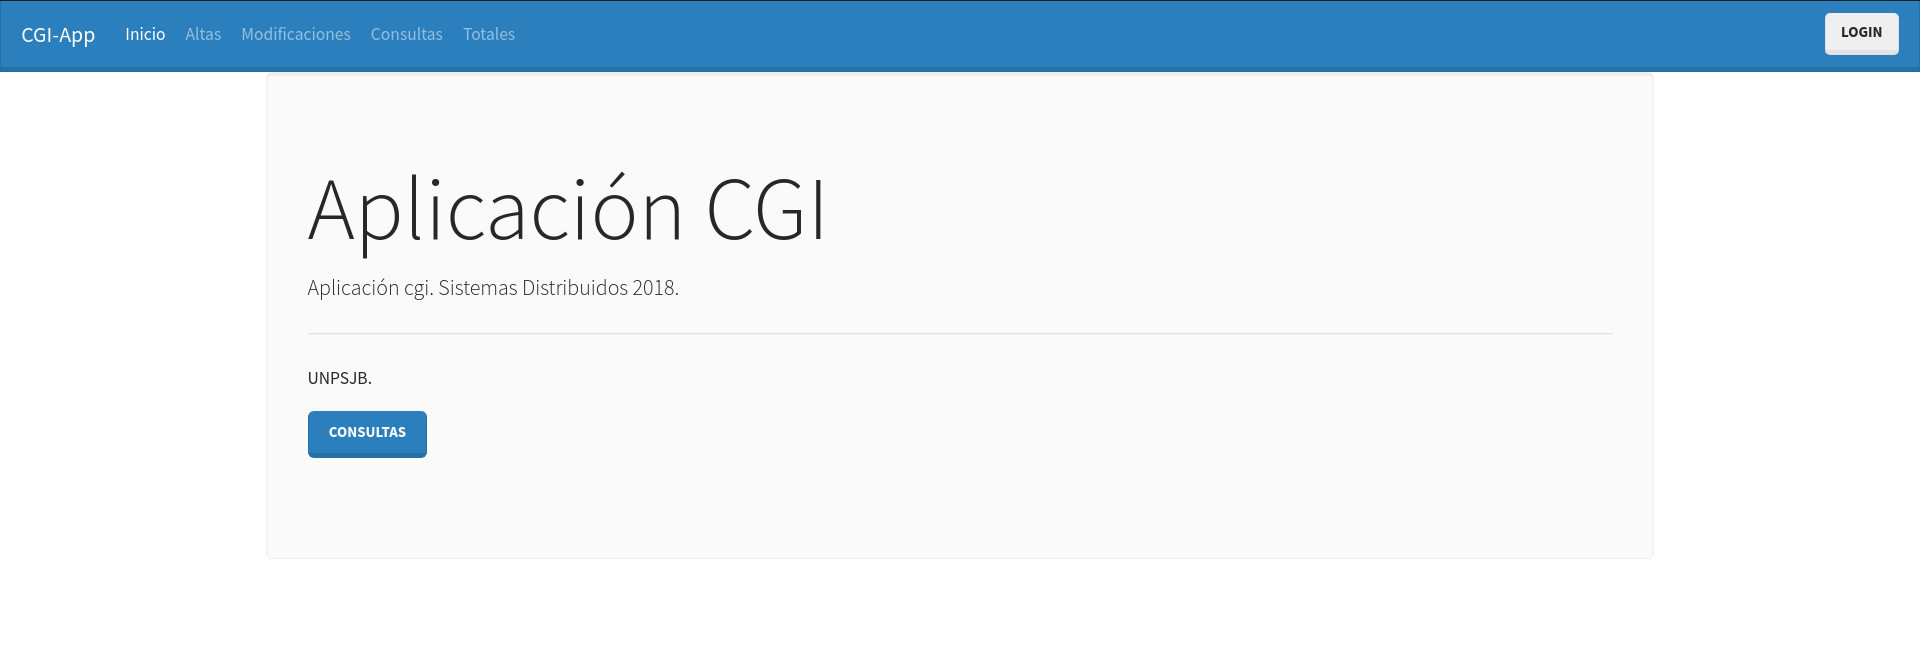
\includegraphics{images/interfaz-cgi.png}
\caption{}
\end{figure}

\subsection{Conclusion}\label{conclusion}

Esta aplicacion que se implemento puede ser considerada una aplicacion
web ya que cumple todos sus fundamentos.

El cliente (navegador) para cada llamada a un servicio del servidor
realiza una llamada \textbf{cgi} hacia el servidor (que son scripts cgi
que residen en el servidor)y el mismo responde de acuerdo a la peticion
realizada.

    \section{Agregue a la aplicación del ejercicio 3 cuatro posibilidades de
consultas básicas: por nombre y apellido (pueden haber ``*''), Número de
Alumno/Legajo (puede ser un intervalo), sexo, y edad (puede ser un
intervalo). Los resultados deben mostrarse visualmente
diferenciados}\label{agregue-a-la-aplicaciuxf3n-del-ejercicio-3-cuatro-posibilidades-de-consultas-buxe1sicas-por-nombre-y-apellido-pueden-haber-nuxfamero-de-alumnolegajo-puede-ser-un-intervalo-sexo-y-edad-puede-ser-un-intervalo.-los-resultados-deben-mostrarse-visualmente-diferenciados}

\textbf{COMENTARIO:} este ejercicio es para que se vea que el programa
CGI debería combinar la generación de HMTL con el resultado de lo que se
procesa localmente en el servidor. Y que el HTML generado puede ser
"largo". El programa CGI puede estar en el lenguaje que se desee.

    \subsection{Solucion}\label{solucion}

Para la solucion de este punto, se decidio agregar en la aplicacion un
apartado para \textbf{consultas} en el cual se despliega un formulario
para ingresar el/los filtros para realizar la busqueda.

Como se menciono anteriormente, se utilizo la libreria de python
\textbf{pandas} para el manejo de los archivos \textbf{.csv} para asi
poder manupularlos de una manera mas facil y menos rudimentaria.

\begin{figure}[h]
\centering
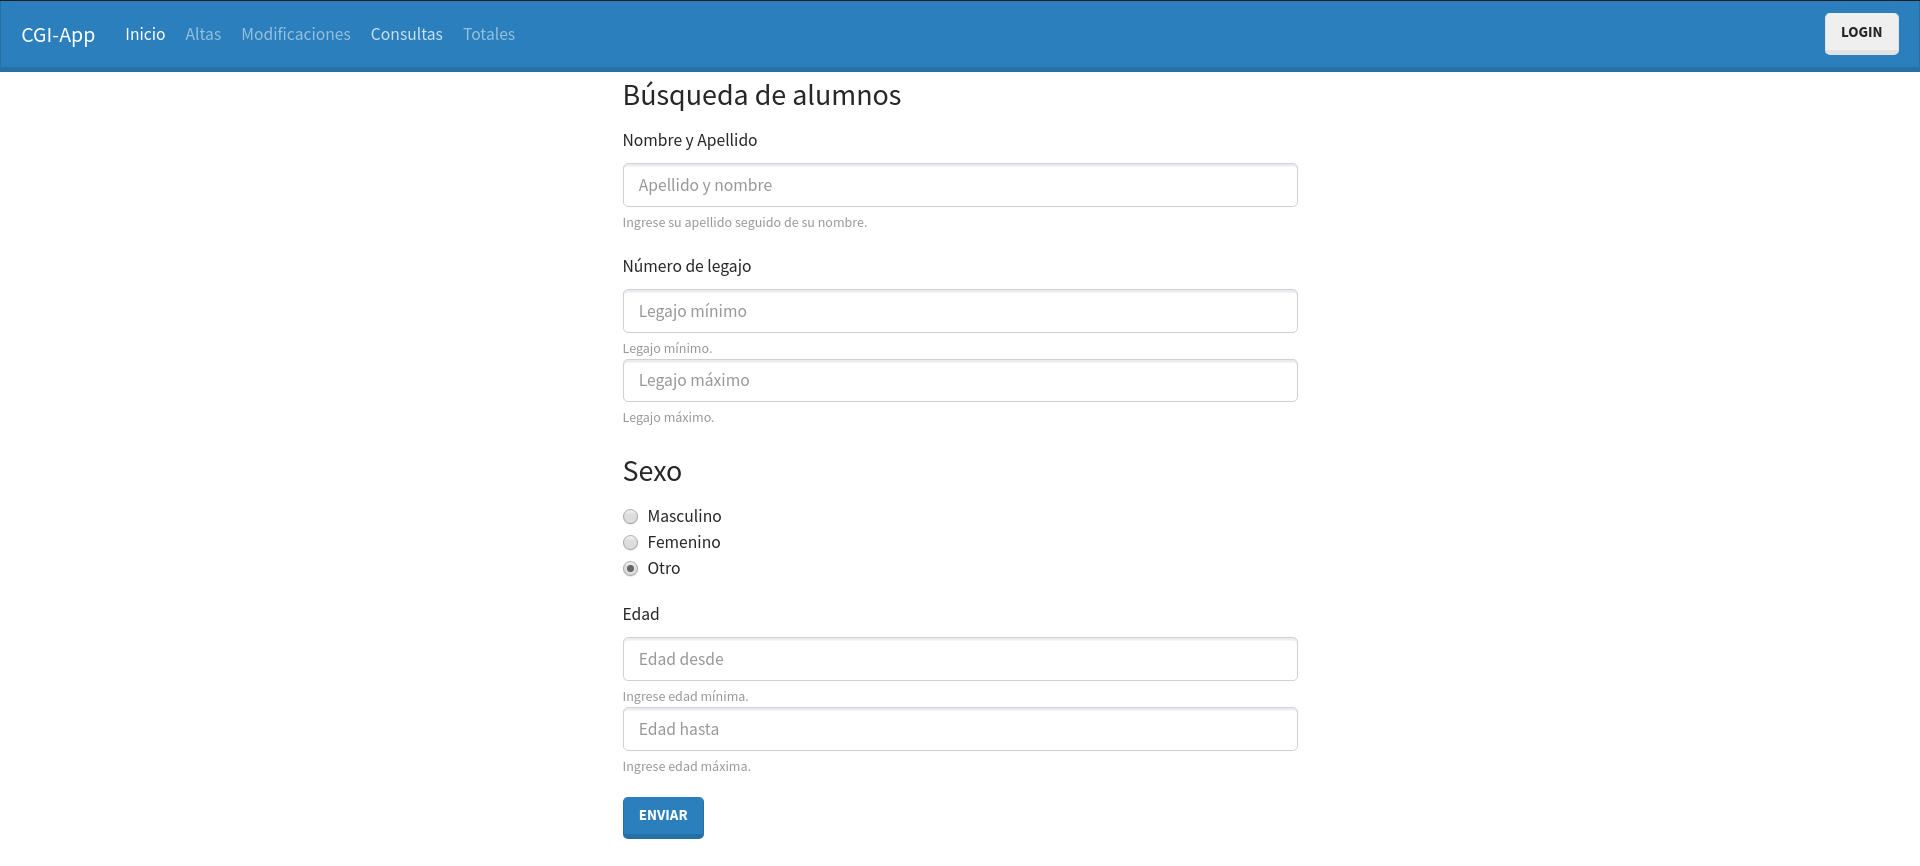
\includegraphics{images/consultas.png}
\caption{}
\end{figure}

    \section{Agregue a la aplicación la consulta de valores totales por
rango de edad (0-20, 20-40, mas de 40) y
sexo.}\label{agregue-a-la-aplicaciuxf3n-la-consulta-de-valores-totales-por-rango-de-edad-0-20-20-40-mas-de-40-y-sexo.}

\textbf{COMENTARIO:} este ejercicio es para que se vea que la mayor
parte del procesamiento en el lado del servidor puede ser solamente para
computar valores simples a mostrar, pero que pueden ser resultado de
procesamiento relativamente complejo.

    \subsection{Impleentacion}\label{impleentacion}

De la misma forma que se hizo con las consultas del punto anterior, para
este caso se agrego un apartado \textbf{totales} a nuestra aplicacion en
la cual se muestra como resultado una tabla con los totales por rango de
edad y sexo.

La resolucion tambien fue realizada con la libreria de python
\textbf{pandas}.

\begin{Shaded}
\begin{Highlighting}[]
\KeywordTok{def}\NormalTok{ get_totales(cls):}
\NormalTok{    alumnos }\OperatorTok{=}\NormalTok{ pd.read_csv(MODEL_FILE)}

\NormalTok{    result }\OperatorTok{=}\NormalTok{ \{}
        \StringTok{"mujeres1"}\NormalTok{:}\BuiltInTok{len}\NormalTok{(alumnos[(alumnos[}\StringTok{'sexo'}\NormalTok{] }\OperatorTok{==} \StringTok{"femenino"}\NormalTok{) }\OperatorTok{&} \OperatorTok{\textbackslash{}}
\NormalTok{                               (alumnos[}\StringTok{'edad'}\NormalTok{] }\OperatorTok{<} \DecValTok{21}\NormalTok{)]),}
        \StringTok{"mujeres2"}\NormalTok{:}\BuiltInTok{len}\NormalTok{(alumnos[(alumnos[}\StringTok{'sexo'}\NormalTok{] }\OperatorTok{==} \StringTok{"femenino"}\NormalTok{) }\OperatorTok{&} \OperatorTok{\textbackslash{}}
\NormalTok{                               ((alumnos[}\StringTok{'edad'}\NormalTok{] }\OperatorTok{>} \DecValTok{20}\NormalTok{) }\OperatorTok{&}\NormalTok{ (alumnos[}\StringTok{'edad'}\NormalTok{] }\OperatorTok{<} \DecValTok{41}\NormalTok{))]),}
        \StringTok{"mujeres3"}\NormalTok{:}\BuiltInTok{len}\NormalTok{(alumnos[(alumnos[}\StringTok{'sexo'}\NormalTok{] }\OperatorTok{==} \StringTok{"femenino"}\NormalTok{) }\OperatorTok{&} \OperatorTok{\textbackslash{}}
\NormalTok{                               (alumnos[}\StringTok{'edad'}\NormalTok{] }\OperatorTok{>} \DecValTok{40}\NormalTok{)]),}
        \StringTok{"varones1"}\NormalTok{:}\BuiltInTok{len}\NormalTok{(alumnos[(alumnos[}\StringTok{'sexo'}\NormalTok{] }\OperatorTok{==} \StringTok{"masculino"}\NormalTok{) }\OperatorTok{&} \OperatorTok{\textbackslash{}}
\NormalTok{                               (alumnos[}\StringTok{'edad'}\NormalTok{] }\OperatorTok{<} \DecValTok{21}\NormalTok{)]),}
        \StringTok{"varones2"}\NormalTok{:}\BuiltInTok{len}\NormalTok{(alumnos[(alumnos[}\StringTok{'sexo'}\NormalTok{] }\OperatorTok{==} \StringTok{"masculino"}\NormalTok{) }\OperatorTok{&} \OperatorTok{\textbackslash{}}
\NormalTok{                               ((alumnos[}\StringTok{'edad'}\NormalTok{] }\OperatorTok{>} \DecValTok{20}\NormalTok{) }\OperatorTok{&}\NormalTok{ (alumnos[}\StringTok{'edad'}\NormalTok{] }\OperatorTok{<} \DecValTok{41}\NormalTok{))]),}
        \StringTok{"varones3"}\NormalTok{:}\BuiltInTok{len}\NormalTok{(alumnos[(alumnos[}\StringTok{'sexo'}\NormalTok{] }\OperatorTok{==} \StringTok{"masculino"}\NormalTok{) }\OperatorTok{&} \OperatorTok{\textbackslash{}}
\NormalTok{                               (alumnos[}\StringTok{'edad'}\NormalTok{] }\OperatorTok{>} \DecValTok{40}\NormalTok{)]),}
        \StringTok{"otro1"}\NormalTok{:}\BuiltInTok{len}\NormalTok{(alumnos[(alumnos[}\StringTok{'sexo'}\NormalTok{] }\OperatorTok{==} \StringTok{"otro"}\NormalTok{) }\OperatorTok{&} \OperatorTok{\textbackslash{}}
\NormalTok{                            (alumnos[}\StringTok{'edad'}\NormalTok{] }\OperatorTok{<} \DecValTok{21}\NormalTok{)]),}
        \StringTok{"otro2"}\NormalTok{:}\BuiltInTok{len}\NormalTok{(alumnos[(alumnos[}\StringTok{'sexo'}\NormalTok{] }\OperatorTok{==} \StringTok{"otro"}\NormalTok{) }\OperatorTok{&} \OperatorTok{\textbackslash{}}
\NormalTok{                            ((alumnos[}\StringTok{'edad'}\NormalTok{] }\OperatorTok{>} \DecValTok{20}\NormalTok{) }\OperatorTok{&}\NormalTok{ (alumnos[}\StringTok{'edad'}\NormalTok{] }\OperatorTok{<} \DecValTok{41}\NormalTok{))]),}
        \StringTok{"otro3"}\NormalTok{:}\BuiltInTok{len}\NormalTok{(alumnos[(alumnos[}\StringTok{'sexo'}\NormalTok{] }\OperatorTok{==} \StringTok{"otro"}\NormalTok{) }\OperatorTok{&} \OperatorTok{\textbackslash{}}
\NormalTok{                            (alumnos[}\StringTok{'edad'}\NormalTok{] }\OperatorTok{>} \DecValTok{40}\NormalTok{)]),}
\NormalTok{    \}}

    \ControlFlowTok{return}\NormalTok{ result}
\end{Highlighting}
\end{Shaded}

\subsection{Vista desde la aplicacion}\label{vista-desde-la-aplicacion}

\begin{figure}[h]
\centering
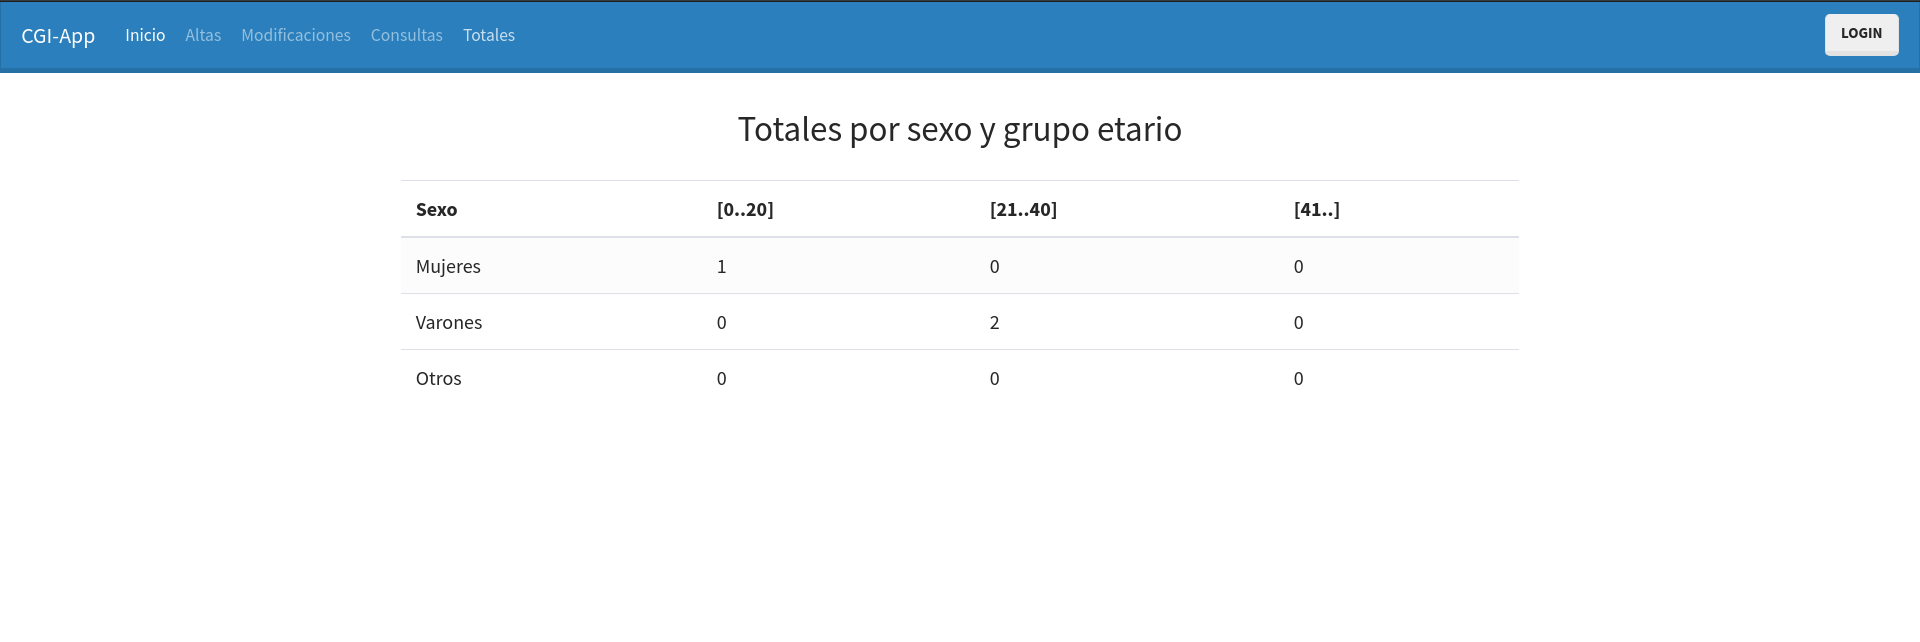
\includegraphics{images/totales.png}
\caption{}
\end{figure}

    \section{Tome el código que se adjunta como Anexo 5 del apunte de AJAX y
agregue las siguientes mejora de
funcionalidad:}\label{tome-el-cuxf3digo-que-se-adjunta-como-anexo-5-del-apunte-de-ajax-y-agregue-las-siguientes-mejora-de-funcionalidad}

\begin{itemize}
\item
  \textbf{a)} Agregar un botón a la ventana principal de chat, a efectos
  que un usuario ingresante pueda registrarse en el sitio. El usuario
  ingresará su ``Nick'' y al pulsar el botón, se registrará en un
  archivo data/usuarios.txt en el servidor.
\item
  \textbf{b)} Producido el registro, se devolverá al usuario una lista
  total de usuarios registrados en una pequeña ventana a la derecha de
  la ventana común de mensajes y también se devolverá toda la
  conversación entre usuarios registrada hasta ese momento.
\item
  \textbf{c)} Intentar establecer la actualización incremental del chat,
  mediante el almacenamiento en cada cliente de la última línea de chat
  enviada.
\end{itemize}

    \subsection{Diseño e implementación del
servidor}\label{diseuxf1o-e-implementaciuxf3n-del-servidor}

\subsubsection{Modelos}\label{modelos}

Se definieron dos modelos que resuelven la lógica de negocio de la
aplicación. Por un lado la clase Session (similar a la implementada en
el ejercicio anterior) y por otro la clase Message.

La clase Session posee los siguientes atributos:

\begin{Shaded}
\begin{Highlighting}[]
\VariableTok{self}\NormalTok{.}\BuiltInTok{id} \CommentTok{# identificador único autoincremental para manejo del archivo}
\VariableTok{self}\NormalTok{.nickname }\CommentTok{# nickname del usuario }
\VariableTok{self}\NormalTok{.cookie }\CommentTok{# objeto cookie}
\VariableTok{self}\NormalTok{.last_msg }\CommentTok{# identificador del último mensaje entregado al usuario}
\end{Highlighting}
\end{Shaded}

y los siguientes métodos

\begin{Shaded}
\begin{Highlighting}[]
\KeywordTok{def}\NormalTok{ save(}\VariableTok{self}\NormalTok{): }
\CommentTok{# guarda una sessión en el archivo}
\KeywordTok{def}\NormalTok{ update(}\VariableTok{self}\NormalTok{, last_msg): }
\CommentTok{# actializa el id del último mensaje entregado al usuario}
\KeywordTok{def}\NormalTok{ _new_cookie(}\VariableTok{self}\NormalTok{): }
\CommentTok{# genera una nueva cookie de sesión}
\KeywordTok{def}\NormalTok{ delete_cookie(}\VariableTok{self}\NormalTok{): }
\CommentTok{# elimina una cookie y borra la sesión del registro}
    
\AttributeTok{@classmethod}
\KeywordTok{def}\NormalTok{ get_users(cls, nickname): }
\CommentTok{# obtiene la lista de usuarios conectados}
\AttributeTok{@classmethod}
\KeywordTok{def}\NormalTok{ get_current_session(cls): }
\CommentTok{# devuelve una instancia de Session que representa la sesión actual}
\AttributeTok{@classmethod}
\KeywordTok{def}\NormalTok{ exists(cls): }
\CommentTok{# chequea si existe una sesión}
\end{Highlighting}
\end{Shaded}

Los atributos de la clase Message son:

\begin{Shaded}
\begin{Highlighting}[]
\VariableTok{self}\NormalTok{.}\BuiltInTok{id} \CommentTok{# identificador único autoincremental para manejo del archivo}
\VariableTok{self}\NormalTok{.user }\CommentTok{# nickname del usuario que envió el mensaje}
\VariableTok{self}\NormalTok{.text }\CommentTok{# texto del mensaje}
\end{Highlighting}
\end{Shaded}

y tiene los siguientes métodos:

\begin{Shaded}
\begin{Highlighting}[]
\KeywordTok{def}\NormalTok{ save(}\VariableTok{self}\NormalTok{):}
\CommentTok{# guarda un mensaje en el archivo}

\AttributeTok{@classmethod}
\KeywordTok{def}\NormalTok{ get_messages(cls, last_msg_id}\OperatorTok{=}\VariableTok{None}\NormalTok{):}
\CommentTok{# Obtiene una colección de mensajes, desde last_msg_id en adelante }
\CommentTok{# o desde 0 si last_msg_id es None}

\AttributeTok{@classmethod}
\KeywordTok{def}\NormalTok{ get_last_msg_id(cls):}
\CommentTok{# obtiene el id del último mensaje registrado en el archivo}
\end{Highlighting}
\end{Shaded}

\subsubsection{Controladores}\label{controladores}

Los controladores de la aplicación se encuentran definidos en los
siguientes archivos:

\begin{Shaded}
\begin{Highlighting}[]
\NormalTok{login.py }
\CommentTok{# maneja peticiones post login}
\NormalTok{logout.py }
\CommentTok{# maneja peticiones post logout}
\NormalTok{messages.py }
\CommentTok{# maneja peticiones get para obtener mensajes y post para guardarlos}
\NormalTok{users.py }
\CommentTok{# maneja peticiones get para obtener los usuarios conectados}
\NormalTok{main.py }
\CommentTok{# recibe un get y resuelve mostrar la vista login o chat }
\CommentTok{# según usuario autenticado }
\end{Highlighting}
\end{Shaded}

\subsection{Diseño e implementación del
cliente}\label{diseuxf1o-e-implementaciuxf3n-del-cliente}

Similarmente a como se resolvió en el ejercicio anterior, la aplicación
tiene una sola página (index.html) y vía ajax se carga el contenido
dinámicamente en el div principal (id="frame"):

\begin{Shaded}
\begin{Highlighting}[]
\KeywordTok{<body>}
  \KeywordTok{<div}\OtherTok{ class=}\StringTok{"container-fluid"}\KeywordTok{>}
    \KeywordTok{<div}\OtherTok{ class=}\StringTok{"row justify-content-md-center frame"}\KeywordTok{>}
      \KeywordTok{<div}\OtherTok{ id=}\StringTok{"frame"}\KeywordTok{>}
        
      \KeywordTok{</div>}
    \KeywordTok{</div>}
  \KeywordTok{</div>}
\KeywordTok{</body>}
\end{Highlighting}
\end{Shaded}

\subsubsection{Controladores del
cliente}\label{controladores-del-cliente}

Las peticiones post a las rutas \emph{cgi-bin/login.py},
\emph{cgi-bin/logout.py} y \emph{cgi-bin/messages.py} son gestionadas
por los scripts:

\begin{Shaded}
\begin{Highlighting}[]
\VariableTok{login}\NormalTok{.}\AttributeTok{js} 
\VariableTok{logout}\NormalTok{.}\AttributeTok{js}
\VariableTok{send_message}\NormalTok{.}\AttributeTok{js}
\end{Highlighting}
\end{Shaded}

Su funcioanmiento es similar en los 3 casos.

Al cargarse la página se ejecuta el script definido en \emph{main.js}
que lanzará la primera petición get a la ruta \emph{cgi-bin/main.py}:

\begin{Shaded}
\begin{Highlighting}[]
\AttributeTok{\$}\NormalTok{( document ).}\AttributeTok{ready}\NormalTok{(}\KeywordTok{function}\NormalTok{()}\OperatorTok{\{}
    
    \AttributeTok{main}\NormalTok{()}\OperatorTok{;}
    \KeywordTok{function} \AttributeTok{main}\NormalTok{()}\OperatorTok{\{}
        \KeywordTok{var}\NormalTok{ container }\OperatorTok{=}\NormalTok{  (}\StringTok{"#frame"}\NormalTok{)}
\NormalTok{        .}\AttributeTok{ajax}\NormalTok{(}\OperatorTok{\{}
            \DataTypeTok{method}\OperatorTok{:} \StringTok{"GET"}\OperatorTok{,}
            \DataTypeTok{url}\OperatorTok{:} \StringTok{"/cgi-bin/main.py"}\OperatorTok{,}
        \OperatorTok{\}}\NormalTok{)}
\NormalTok{        .}\AttributeTok{done}\NormalTok{(}\KeywordTok{function}\NormalTok{ (res) }\OperatorTok{\{}
            \VariableTok{container}\NormalTok{.}\AttributeTok{html}\NormalTok{(res)}\OperatorTok{;}
        \OperatorTok{\}}\NormalTok{)}
\NormalTok{        .}\AttributeTok{fail}\NormalTok{(}\KeywordTok{function}\NormalTok{ (err) }\OperatorTok{\{}
            \VariableTok{container}\NormalTok{.}\AttributeTok{html}\NormalTok{(err)}\OperatorTok{;}
        \OperatorTok{\}}\NormalTok{)}\OperatorTok{;} 
    \OperatorTok{\}}
\OperatorTok{\}}\NormalTok{)}\OperatorTok{;}
\end{Highlighting}
\end{Shaded}

En ese mismo script se verifica si existe una cookie, en caso de existir
se intentará obtener del servidor los mensajes y los usuarios conectados
(si no está autenticado el usuario, éste devolverá error). Esto último
es parte de lo que debe consultarse periódicamente y por eso se define
dentro de una función que engloba estas dos tareas y que se ejecuta cada
2 seg.

\begin{Shaded}
\begin{Highlighting}[]
\KeywordTok{var}\NormalTok{ interval }\OperatorTok{=} \KeywordTok{null}\OperatorTok{;}
\KeywordTok{let}\NormalTok{ cookie }\OperatorTok{=} \VariableTok{Cookies}\NormalTok{.}\AttributeTok{get}\NormalTok{(}\StringTok{'session'}\NormalTok{)}\OperatorTok{;}

\ControlFlowTok{if}\NormalTok{ (}\KeywordTok{typeof}\NormalTok{ cookie }\OperatorTok{===} \StringTok{"undefined"}\NormalTok{)}\OperatorTok{\{}
    \AttributeTok{clearInterval}\NormalTok{(interval)}\OperatorTok{;}
\OperatorTok{\}} \ControlFlowTok{else} \OperatorTok{\{}       
\NormalTok{    interval }\OperatorTok{=} \AttributeTok{setInterval}\NormalTok{(updateChat}\OperatorTok{,} \DecValTok{2000}\NormalTok{)}\OperatorTok{;}
\OperatorTok{\}}

\KeywordTok{function} \AttributeTok{updateChat}\NormalTok{()}\OperatorTok{\{}
    \AttributeTok{update_messajes}\NormalTok{()}\OperatorTok{;}
    \AttributeTok{update_users}\NormalTok{()}\OperatorTok{;}
\OperatorTok{\}}
\end{Highlighting}
\end{Shaded}

    El resultado final en términos de vistas de la aplicación puede
apreciarse en las siguientes imágenes:

\begin{figure}[h]
\centering
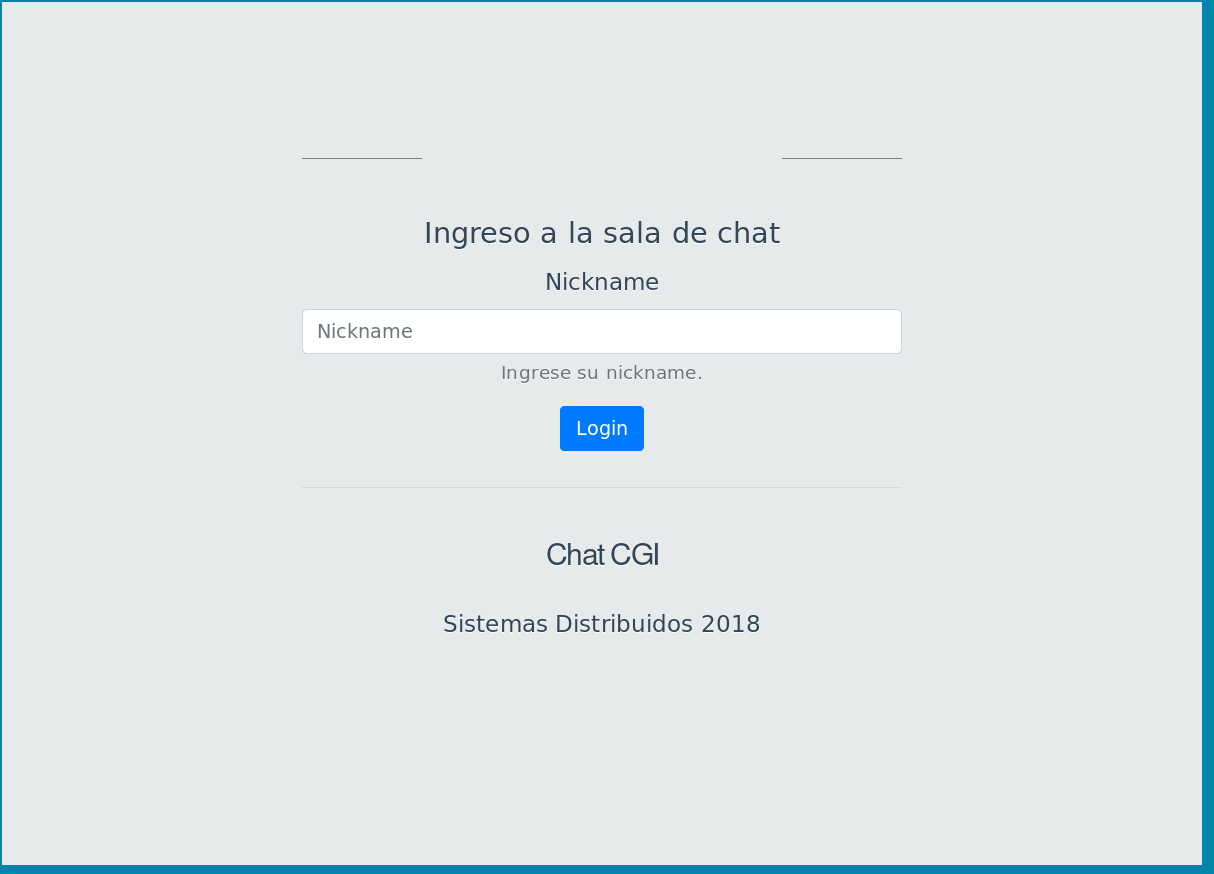
\includegraphics{images/login-chat.png}
\end{figure}

\begin{figure}[h]
\centering
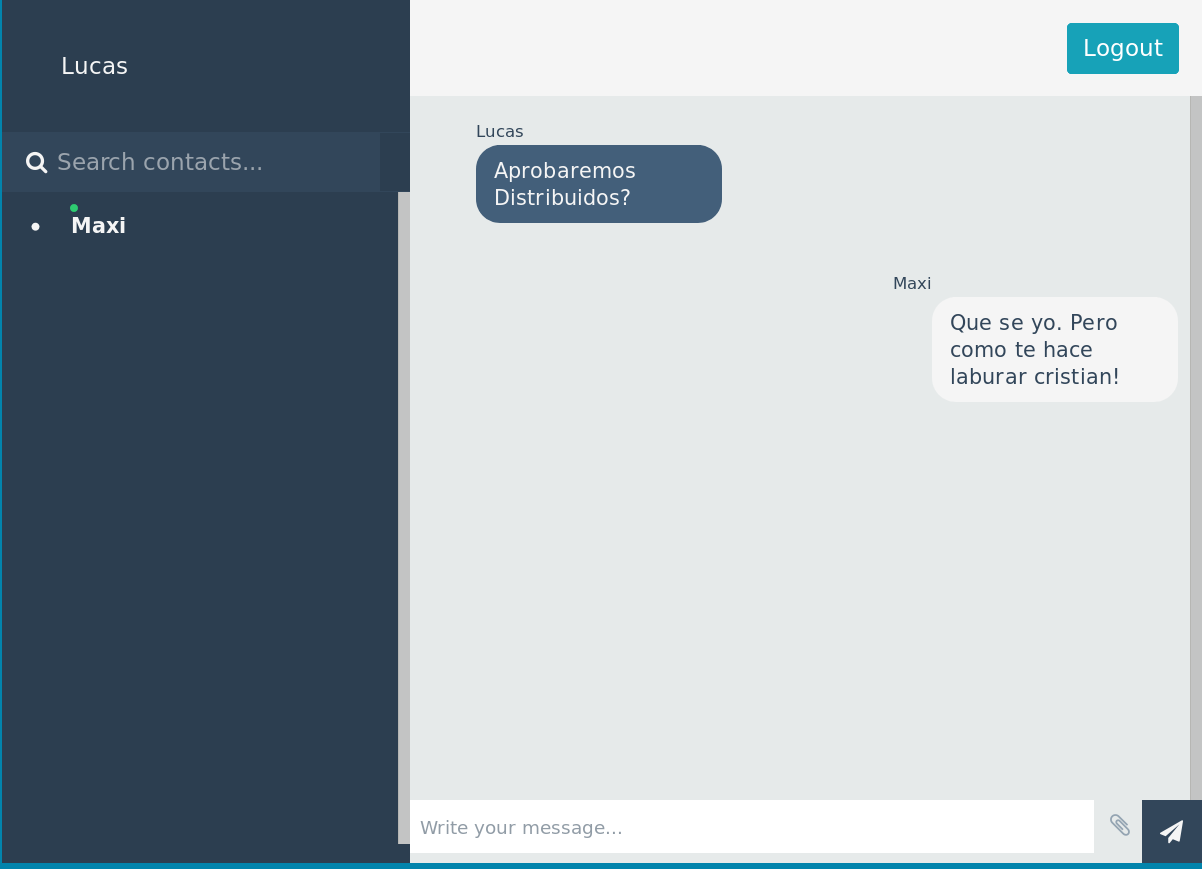
\includegraphics{images/chat-chat.png}
\end{figure}


    \section{DFS:}\label{dfs}

\begin{itemize}
\item
  \textbf{a)} Configurar NFS y efectuar un compartimiento de archivos
  entre un Servidor y un Cliente Linux. Describir la operatoria en el
  informe.
\item
  \textbf{b)} Configurar Samba y efectuar un compartimiento de archivos
  entre un Windows y un Cliente Linux. Describir la operatoria en el
  informe.
\end{itemize}

    \subsection{NFS}\label{nfs}

Un NFS nos permite acceso local a archivos remotos y utiliza una
arquitectura estándar cliente-servidor para compartir archivos entre
maquinas con SO basados en unix. Aún así, no es necesario que las dos
máquinas corran el mismo sistema operativo.

En nuestro caso configuramos NFS para una distribucion ArchLinux.

Como primer paso debemos instalar el paquete \textbf{nfs-utils}.

\begin{verbatim}
sudo pacman -S nfs-utils
\end{verbatim}

\subsubsection{Configuracion}\label{configuracion}

\begin{itemize}
\tightlist
\item
  Iniciar y abilitar los servicios de NFS
\end{itemize}

\begin{verbatim}
systemctl start nfs-server.service
\end{verbatim}

\begin{verbatim}
systemctl enable nfs-server.service
\end{verbatim}

Ahora bien, algunos de los archivos más importantes que entran en juego
con NFS son (Con sus rutas absolutas en ArchLinux): + /etc/exports: Es
el archivo primario de configuración de NFS. Todos los archivos y
carpetas exportados que se especifican en este archivo son los que se
sirven. + /etc/fstab: Archivo de FS de linux en el que se especifican
los puntos de montaje de las diferentes particiones. Se utiliza para
definir un mounpoint para el/los directorio/s de NFS (Y que persistan
luego de reiniciar el sistema). + /etc/idmapd.conf: Archivo en el que se
realiza el mapeo de IDs. Utilizado principalmente para definir el nombre
del dominio para que el servicio se configure correctamente.

\subsubsection{Mapeo de ID}\label{mapeo-de-id}

\begin{itemize}
\item
  Para este paso hay que modificar el archivo de
  configuracion~\textbf{/etc/idmapd.conf}~y establezca el
  campo~\textbf{Domain}~con el nombre de dominio.
\item
  Seguidamente, creamos el recurso que vamos a servir. En este caso es
  una carpeta que ubicaremos en \textbf{/srv/nfs4/datos}
\end{itemize}

\begin{verbatim}
sudo mkdir -p /srv/nfs4/datos
\end{verbatim}

\begin{itemize}
\tightlist
\item
  Luego creamos la carpeta del sistema de archivos del servidor en donde
  será montado el recurso a compartir:
\end{itemize}

\begin{verbatim}
sudo mkdir /mnt/datos
\end{verbatim}

Se deben otorgar permisos de lectura/escritura al directorio
\textbf{datos} para que los clientes puedan escribir en él.

\begin{itemize}
\tightlist
\item
  Luego, como siguiente paso es montar el directorio que desea
  compartir, en este caso~\textbf{/mnt/datos}, en el directorio
  compartido de NFS a través de la instrucción de montaje.
\end{itemize}

\begin{verbatim}
mount --bind /mnt/datos /srv/nfs4/datos
\end{verbatim}

Para hacer que los cambios sean permanentes en cada reinicio del
servidor, añada el enlace de montaje a~\textbf{fstab}

\begin{figure}[h]
\centering

\includegraphics{images/fstab.png}
\caption{}
\end{figure}

\subsubsection{Exportacion}\label{exportacion}

Como siguiente paso, se añaden los directorios que se compartirán y la
dirección IP o nombre de servidor de las máquinas cliente a las que les
estará permitido montarlas en~\textbf{exports}:

\begin{figure}[h]
\centering
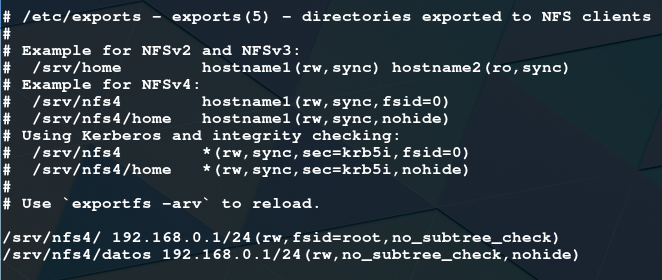
\includegraphics{images/exports.png}
\caption{}
\end{figure}

Si se modifica~\textbf{/etc/exports}~mientras el servidor está
funcionando, debe volver a exportarlos para que los cambios surtan
efecto.

\begin{verbatim}
exportfs -rav
\end{verbatim}

\begin{figure}[h]
\centering
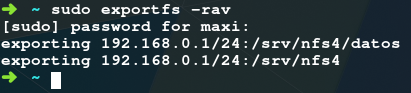
\includegraphics{images/exportfs.png}
\caption{}
\end{figure}

Finalmente, para levantar el servidor, debemos arrancar los servicios
\textbf{rpcbind} y \textbf{nfs-client.target}.

\begin{verbatim}
systemctl start rpcbind nfs-client.target
\end{verbatim}

Ahora desde el lado del \textbf{Cliente}, tambien necesitan el modulo
\textbf{nfs-utils} para poder conectarse.

\subsubsection{Montaje en Linux}\label{montaje-en-linux}

Para mostrar los sistemas de archivos exportados por el servidor:

\begin{verbatim}
showmount -e servername
\end{verbatim}

A continuación se monta omitiendo la raíz de exportación del servidor
NFS:

\begin{verbatim}
mount -t nfs4 servername:/datos /mountpoint/on/client
\end{verbatim}

\subsection{SAMBA}\label{samba}

Como paso inicial debemos instalar el~paquete de~\textbf{samba}.

\begin{verbatim}
sudo pacman -S samba
\end{verbatim}

Samba se configura en el~\textbf{/etc/samba/smb.conf}.

Debido a que el~paquete~samba~no proporciona este archivo, se debe
crear~antes de~iniciar~samba.

Utilizamos un ejemplo documentado~\textbf{smb.conf.default} desde
el~repositorio de git de \textbf{Samba}~para la
configuración~\textbf{/etc/samba/smb.conf}.

Link:
\url{https://git.samba.org/samba.git/?p=samba.git;a=blob_plain;f=examples/smb.conf.default;hb=HEAD}

\begin{itemize}
\tightlist
\item
  Siempre que modifique el~smb.confarchivo, es recomendable ejecutar
  el~comando \textbf{testparm} para verificar si hay errores
  sintácticos.
\end{itemize}

\begin{verbatim}
testparm
\end{verbatim}

\begin{figure}
\centering
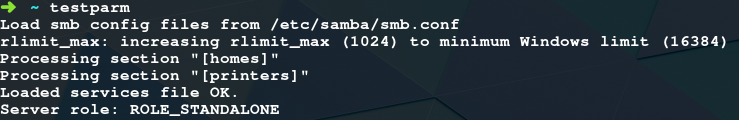
\includegraphics{images/testparm1.png}
\end{figure}

\begin{figure}
\centering
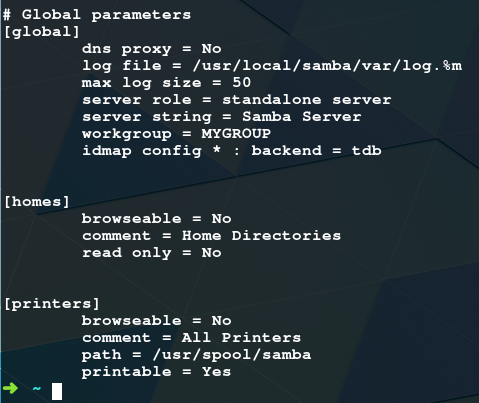
\includegraphics{images/testparm2.png}
\end{figure}

\subsubsection{Gestión de usuarios}\label{gestiuxf3n-de-usuarios}

Samba requiere una cuenta de usuario de Linux. Puede usar una cuenta de
usuario existente o crear una~nueva. Aunque el nombre de usuario se
comparte con el sistema Linux, Samba usa una contraseña separada de la
de las cuentas de usuario de Linux.~Reemplazar~\textbf{samba\_usercon}
la cuenta de usuario Samba elegida:

\begin{verbatim}
smbpasswd -a samba_user
\end{verbatim}

Luego, del lado del cliente (Workgroup del equipo): Debemos asegurarnos
que los servicios smbd y nmbd estén corriendo (Ya sea con START o
ENABLE). Esto inicia la escucha del servidor.

Ahora es necesario crear el recurso compartido. Hacemos una carpeta en
\textbf{/var/lib/samba} llamada \textbf{usershare} (Quedando como:
\textbf{/var/lib/samba/usershare}).

Ahora vamos a modificar los permisos sobre esa carpeta. Típicamente lo
que se hace es crear un grupo de usuarios que se puede llamar
\textbf{sambashare} y se le asignan permisos de lectura/escritura sobre
el recurso compartido. Paso a paso tenemos:

\begin{itemize}
\item
  Creamos el grupo sambashare con el comando \textbf{groupadd -r
  sambashare}
\item
  Cambiamos el grupo dueño de la carpeta compartida con el comando
  ``chown root:sambashare /var/lib/samba/usershare''.
\item
  Cambiamos los permisos a nivel de FS sobre la carpeta compartida con
  el comando ``chmod 770 /var/lib/samba/usershare''
\item
  En el archivo de configuración de samba (smb.conf) debemos agregar el
  recurso compartido. Un posible ejemplo de esto podría ser:

\begin{verbatim}
[global]
 usershare path = /var/lib/samba/usershare
 usershare max shares = 100
 usershare allow guests = yes
 usershare owner only = yes
\end{verbatim}
\end{itemize}

Finalmente, agregamos el usuario al grupo \textbf{sambashare} con el
comando \textbf{gpasswd sambashare -a usuario}. Luego de esto, es
necesario reiniciar la sesión del SO para que se apliquen los cambios.

\begin{verbatim}
gpasswd sambashare -a usuario
\end{verbatim}

    \section{DNS:}\label{dns}

\textbf{Objetivo:} Observar las llamadas implícitas a DNS y ponderar
tiempos de acceso. Efectuar el siguiente experimento, verificando
información con la ayuda de un analizador de protocolo:

\begin{itemize}
\tightlist
\item
  \textbf{a)} Desde el browser haga una conexión a una página WEB de
  argentina, que haya utilizado hace mucho tiempo o que no haya
  utilizado (un diario, un blog, etc.). Obtenga la diferencia temporal
  entre la consulta que se observa en el analizador y su respuesta.
\end{itemize}

\begin{figure}[h]
\centering
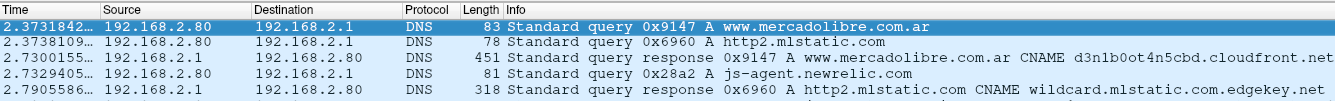
\includegraphics{images/server_nacional.png}
\caption{}
\end{figure}

\begin{itemize}
\tightlist
\item
  \textbf{b)} Haga lo mismo con una página no frecuentada por Ud. que se
  supone que está situada en un servidor europeo o de Asia. (la página
  oficial del grupo Nightwish, o algún diario galés, etc.). Compare sus
  conclusiones con las obtenidas en el caso a).
\end{itemize}

Se puede ver claramente que que el tiempo de respuesta es mucho mayor a
la respuesta a un servidor nacional (como el del anterior caso).

\begin{figure}[h]
\centering
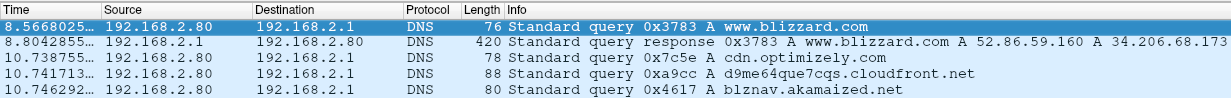
\includegraphics{images/server_externo.png}
\caption{}
\end{figure}

\begin{itemize}
\tightlist
\item
  \textbf{c)} Vuelva nuevamente a invocar la página seleccionada en a),
  (que se supone ya reside en su caché). Compare resultados.
\end{itemize}

Se puede ver la significativa mejora en el tiempo de respuesta de la
peticion, esto es porque la pagina reside en nuestra cache. Siempre que
una pagina resida en la cache, la respuesta sera mucho mas rapida.

\begin{figure}[h]
\centering
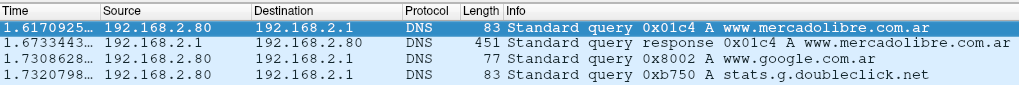
\includegraphics{images/cacheada.png}
\caption{}
\end{figure}

\begin{itemize}
\tightlist
\item
  \textbf{d)} Aporte las conclusiones que puede sacar del experimento.
\end{itemize}

Como pudimos observar en las distintas experiencias, es más rápido
resolver una consulta de una página nacional (www.lanacion.com.ar) que
una europea (www.fortnite.com). Sin embargo los tiempos de respuesta
cambian favorablemente cuando se encuentran cacheadas las páginas, las
respuestas son significativamente mas rapidas.


    % Add a bibliography block to the postdoc
    
    
\bibliographystyle{plain}
\bibliography{references}

    
    \end{document}
